\documentclass{beamer}

\usepackage[utf8]{inputenc}
\usepackage[T1]{fontenc}
\usepackage[english,russian]{babel}
\usepackage{amsmath}
\usepackage{amsfonts}
\usepackage{amssymb}
\usepackage{graphicx,pgf}
\usepackage{multimedia}
\DeclareMathOperator{\tr}{tr}
\usepackage{multirow}
\usepackage{subcaption}

\usetheme{Copenhagen}
%\usetheme{Warsaw}
\useinnertheme{circles}   %внутренняя тема
%\useoutertheme{smoothbars}   %внешняя тема
\usecolortheme{seahorse}     %цветовая схема
%\usefonttheme{serif}    %шрифты
%\defbeamertemplate*{footline}{shadow theme}
%\setbeameroption{hide notes}

%номера слайдов
\newcommand*\oldmacro{}%
\let\oldmacro\insertshorttitle%
\renewcommand*\insertshorttitle{%
	\oldmacro\hfill%
	\insertframenumber\,/\,\inserttotalframenumber}
\RequirePackage{caption}
\DeclareCaptionLabelSeparator{defffis}{ }
\captionsetup{justification=centering,labelsep=defffis}

%\title{Курсовая работа}
%\subtitle{Численные схемы для аппроксимации неограниченных решений при моделировании обтекания профиля крыла в вихревых методах}
\title[Качественно-аналитическое...]{Качественно-аналитическое исследование систем ОДУ}
\author[Швецов Г.А.]{Докладчик: Швецов Г.А.\and\\[0.5mm] Научный руководитель: д.ф-м.н., профессор кафедры ФН-2 Галанин М.П.}

\institute[каф. Прикладная математика ФН-2]{группа ФН2-42Б}
\date{\today}
\titlegraphic{
\includegraphics[width=2cm]{logo.png}}
%\renewcommand{\vec}[1]{\text{\mathversion{bold}${#1}$}}


\begin{document}
	
	\begin{frame}[plain]
		\maketitle
		%\insertshortinstitute{Группа ФН2-41Б}
	\end{frame}
	
	\begin{frame}{Постановка задачи}
\underline{Целью} курсовой работы является исследование, а также рассмотрение задачи Коши для следующей системы ОДУ		
\begin{block}{}
\begin{equation}
	\begin{cases}
	m\dot v=-u\dot m-\alpha m v, \\
	\dot m=-\beta m-\gamma v-f_0, \\
	v=v_0,\,t=0,\\
	m=m_0,\,t=0.
\end{cases}
\label{system1}
\end{equation}
\end{block}
	Данная задача моделирует полет ракеты в среде с трением при заданной начальной скорости и при заданной начальной массе.
	\end{frame}


\section{Линеаризация системы}
	\begin{frame}{Линеаризация системы}
	Из системы (\ref{system1}) получаем одну особую точку $\tilde v=0,\tilde m=-\frac{f_0}{\beta}$.\\
		Перенесем особую точку в начало координат
			\begin{columns}
			\column{0.4\textwidth}
			\begin{block}{Замена переменных}
				\[
				\small
				\begin{cases}
					\xi=v,\\
					\eta=m+\frac{f_0}{\beta}.
				\end{cases}
				\]
			\end{block}
			\column{0.6\textwidth}
			\begin{block}{Нелинейная система}
					\small
					\begin{equation}
							\begin{cases}
							\dot \xi=u\beta+\frac{\beta u}{\beta\eta-f_0}(f_0+\gamma\xi)-\alpha\xi,\\
							\dot \eta=-\gamma \xi -\beta \eta.
						\end{cases}
					\end{equation}
			\end{block}
		\end{columns}
	\medskip
		Линеаризуем и получим \textit{систему первого приближения}
		\begin{columns}
		\column{0.5\textwidth}
	\begin{block}{Линейная система}
			\small
			\begin{equation}
\begin{cases}
	\dot \xi=-(\frac{u\gamma \beta}{f_0}+\alpha)\xi-\frac{u\beta^2}{f_0}\eta,\\
	\dot \eta=-\gamma \xi -\beta \eta.
\end{cases}
			\end{equation}
	\end{block}
		\column{0.5\textwidth}
		\begin{block}{Матрица Якоби}
				\small
				\begin{equation}
	\mathbb{J}=\begin{pmatrix}
	-\frac{u\gamma \beta}{f_0}-\alpha & -\frac{u\beta^2}{f_0} \\
	-\gamma & -\beta
\end{pmatrix}
				\end{equation}
		\end{block}
	\end{columns}
	\end{frame}	
	
		
	\section{Фазовые портреты в зависимости от собственных чисел}
	\begin{frame}{Фазовые портреты в зависимости от собственных чисел}
	Для матрицы Якоби $\mathbb{J}$ найдем собственные числа
\begin{block}{}
\[
	\lambda_{1,2}=\frac{1}{2}\left(-\alpha-\beta-\frac{u\beta\gamma}{f_0}\pm\sqrt{-4\alpha\beta+\left(\alpha+\beta+\frac{u\beta\gamma}{f_0}\right)^2}\right)
\]
\end{block}
\begin{table}[H]
	\centering		
		\captionsetup{labelformat=empty}
	\caption{Классификация точек покоя}
	\begin{tabular}{|c|c|}
		\hline
		Корни  & Тип точки покоя \\
		\hline
		$\lambda_1,\,\lambda_2\in\mathbb{R}\text{, } \lambda_1\lambda_2=\alpha\beta>0$& Узел\\
		\hline
		$\lambda_1,\,\lambda_2\in\mathbb{R}\text{, } \lambda_1\lambda_2=\alpha\beta<0$& Седло\\
		\hline
		$\lambda_1,\,\lambda_2\in\mathbb{C}\text{, }\operatorname{Re}(\lambda_1)=\operatorname{Re}(\lambda_2)\ne0$ & Фокус\\
		\hline
		$\lambda_1,\,\lambda_2\in\mathbb{C}\text{, }\operatorname{Re}(\lambda_1)=\operatorname{Re}(\lambda_2)=0$ & Центр\\
		\hline	
	\end{tabular}
\end{table}	
	\end{frame}

%	\section{Фазовые портреты в зависимости от параметров}
%\begin{frame}{Фазовые портреты в зависимости от параметров}
%С помощью матрицы Якоби $\mathbb{J}$ можно определить тип точки покоя и характер ее устойчивости, зная только ее след $\tr \mathbb{J}$ и	определитель $\det \mathbb{J}$.
%\begin{block}{}
%\[
%\small
%\det \mathbb{J} =\begin{vmatrix}
%	-\frac{u\gamma \beta}{f_0}-\alpha & -\frac{u\beta^2}{f_0} \\
%	-\gamma & -\beta
%\end{vmatrix}=
%\alpha \beta,
%\quad
%\tr \mathbb{J}=-\alpha-\beta-\frac{u\gamma \beta}{f_0}.
%\]
%\end{block}
%	\begin{table}[H]
%		\tiny
%		\centering		
%		\begin{tabular}{|c|c|c|c|}
%			\hline
%			\textbf{Определитель матрицы} & \textbf{След матрицы} & \textbf{Тип точки покоя} \\
%			\hline
%			$\alpha\beta<0$ & --- & Седло\\
%			\hline
%			\multirow{2}{*}{$0<4\alpha\beta<(\alpha+\beta+\frac{u\gamma\beta}{f_0})^2$} 
%			&$\tr\mathbb{J}<0$  & Устойчивый узел (УУ)\\
%			\cline {2-3} & $\tr\mathbb{J}>0$ & Неустойчивый узел (НУ)\\
%			\hline
%			\multirow{2}{*}{$4\alpha\beta=(\alpha+\beta+\frac{u\gamma\beta}{f_0})^2$} & $\tr\mathbb{J}<0$ & Дикритический или вырожденный УУ \\
%			\cline {2-3} & $\tr\mathbb{J}>0$ & Дикритический или вырожденный НУ \\
%			\hline
%			\multirow{3}{*}{$4\alpha\beta>(\alpha+\beta+\frac{u\gamma\beta}{f_0})^2$} 
%			&$\tr\mathbb{J}<0$  & Устойчивый фокус (УФ)\\
%			\cline {2-3} & $\tr\mathbb{J}=0$ & Центр\\
%			\cline {2-3} & $\tr\mathbb{J}>0$ & Неустойчивый фокус (НФ)\\
%			\hline
%		\end{tabular}
%	\end{table}	
%\end{frame}

\section{Исследование устойчивости точки покоя}
\begin{frame}{Исследование устойчивости точки покоя}
		\centering
	\large
	Невырожденный узел
	$f_0=2,\,\alpha=3,\,\beta=4,\,\gamma=3,\,u=1$
	\begin{figure}[H]
		\centering
		\begin{subfigure}[H]{0.4\textwidth}
			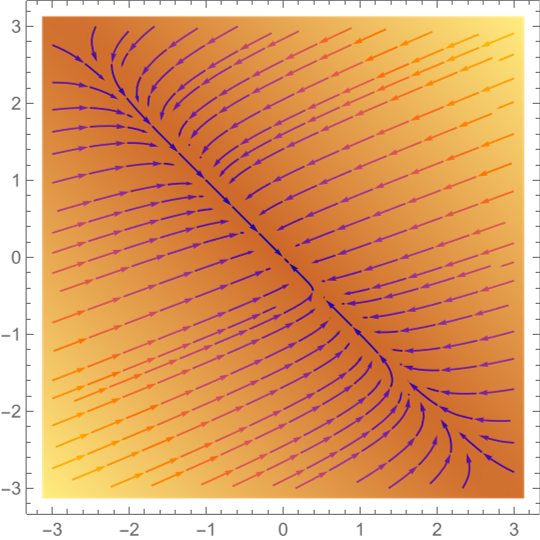
\includegraphics[width=\textwidth]{p1_2_1}
			\captionsetup{labelformat=empty}
			\caption{Фазовый портрет линейной системы}
		\end{subfigure}
		\qquad\qquad
		\begin{subfigure}[H]{0.4\textwidth}
			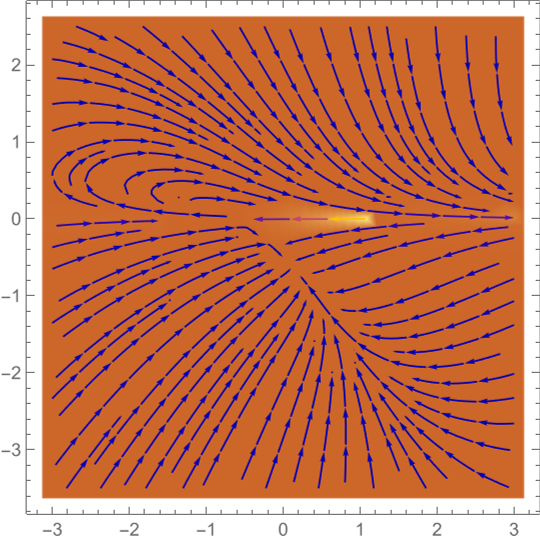
\includegraphics[width=\textwidth]{p1_2_2}
			\captionsetup{labelformat=empty}
			\caption{Фазовый портрет нелинейной системы}
		\end{subfigure}	
	\end{figure}
\end{frame}

\begin{frame}{Исследование устойчивости точки покоя}
	\centering
	\large
	Центр
	$f_0=-2,\,\alpha=4,\,\beta=4,\,\gamma=2,\,u=1$
		\begin{figure}[H]
		\centering
		\begin{subfigure}[H]{0.4\textwidth}
			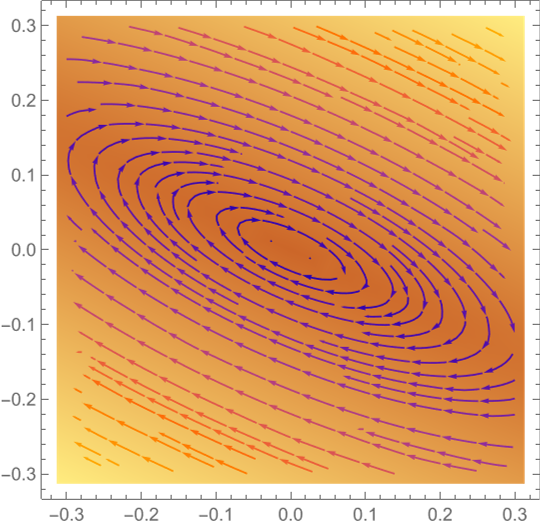
\includegraphics[width=\textwidth]{p6}
			\captionsetup{labelformat=empty}
			\caption{Фазовый портрет линейной системы}
		\end{subfigure}
		\qquad\qquad
		\begin{subfigure}[H]{0.4\textwidth}
			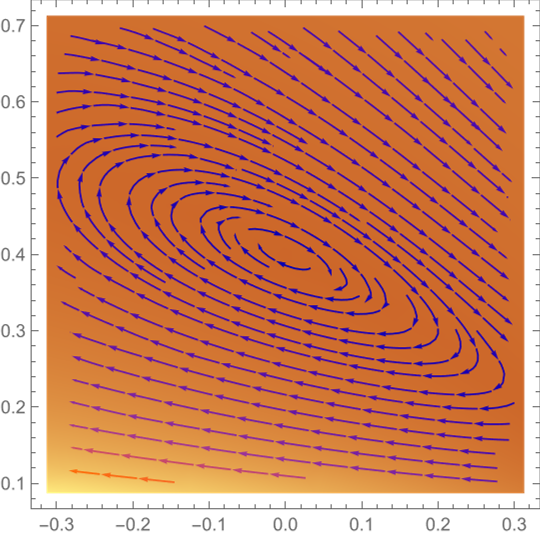
\includegraphics[width=\textwidth]{p66}
			\captionsetup{labelformat=empty}
			\caption{Фазовый портрет нелинейной системы}
		\end{subfigure}	
	\end{figure}
\end{frame}

\section{Аналитическое решение системы}
\begin{frame}{Аналитическое решение системы}
		Для нахождения аналитического решения предположим, что $\gamma=f_0=0$. Тогда перепишем систему (\ref{system1}) в виде
		\begin{block}{}
	\begin{equation}
	\begin{cases}
		\dot v=u\beta-\alpha v, \\
		\dot m=-\beta m, \\
		v=v_0,\,t=0,\\
		m=m_0,\,t=0.
	\end{cases}
	\label{system7}
\end{equation}
		\end{block}
	Получим частное решение системы (\ref{system7})
		\begin{block}{}
			\[
			\begin{cases}
			v=\frac{u\beta+(\alpha v_0-u\beta)e^{-\alpha t}}{\alpha},\\
			m=m_0e^{-\beta t}.
			\end{cases}
			\]
		\end{block}
\end{frame}
	
	\begin{frame}{Аналитическое решение системы}
	Графическое представление частного решения системы
\begin{figure}[H]
	\centering
	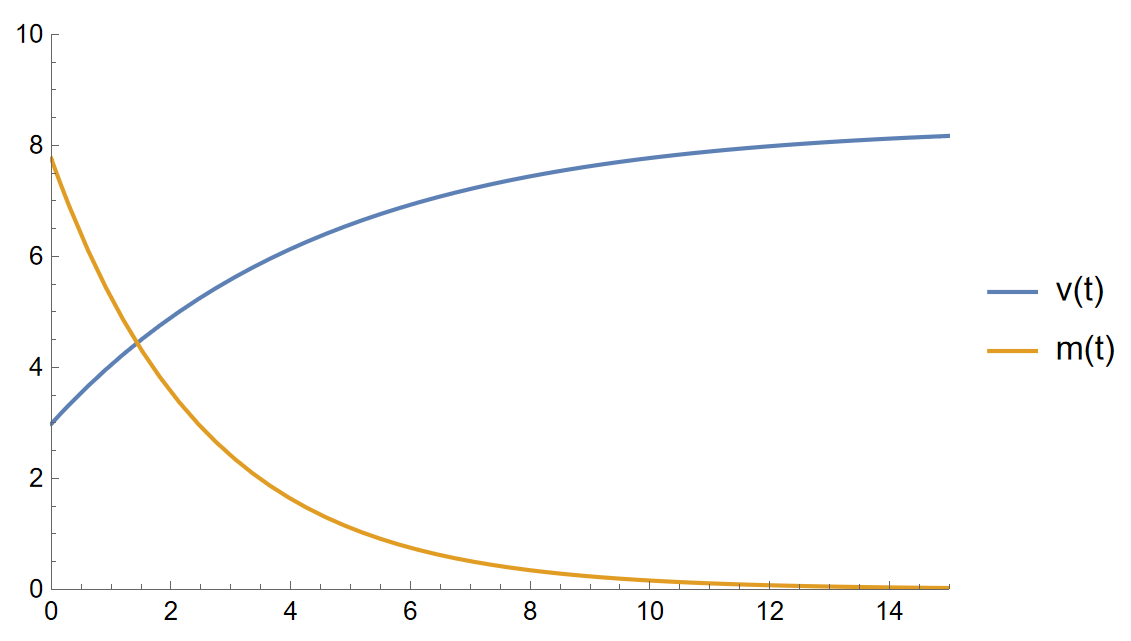
\includegraphics[width=10cm]{graphic}
\end{figure}	
	\end{frame}
			\begin{frame}{Результаты}
				\Large
				В ходе работы получены следующие результаты
				\begin{block}{}
					\begin{enumerate}
						\Large
						\item изучена линеаризация нелинейных систем;
						\item исследована устойчивость точки покоя в зависимости от параметров задачи;
						\item найдено аналитическое решение системы ОДУ.
					\end{enumerate}
				\end{block}	
			\end{frame}	
		\begin{frame}
			\LARGE\center
			Спасибо за внимание!
		\end{frame}
		\end{document} 